\section{Data value}

A data architecture outlines how data is managed throughout its lifecycle, from collection to transformation, distribution, and consumption. 
It serves as a blueprint for how data flows through various storage systems, ensuring that it is processed and delivered effectively.

In traditional data architectures, the process follows the Extract, Transform, Load (ETL) model. 
This method involves extracting data from sources, transforming it into a usable format, and then loading it into a data warehouse for storage and analysis.

However, modern data architectures have shifted to the Extract, Load, Transform (ELT) approach. 
Instead of transforming all data before storing it in a warehouse, raw data is directly placed in a data lake. 
From there, data can be analyzed as needed. 
This approach is more flexible and enables real-time analytics, allowing organizations to process and analyze data on the fly, rather than waiting for a full transformation process to complete.

\subsection{Project}
\begin{definition}[\textit{Project}]
    A project is a set of tasks that must be completed within a defined timeline to accomplish a specific set of goals.
\end{definition}
\noindent A project is defined by its scope, which outlines the goals, deliverables, and constraints. 
    It involves multiple stakeholders and is executed by a project team. 
    The project's methodology, which serves as a framework for executing and managing the project, includes processes, methods, and best practices to ensure that project objectives are met.
\begin{enumerate}
    \item \textit{Waterfall}: in the waterfall methodology, projects are completed in a linear, sequential manner. 
        Each phase depends on the completion of the previous one. 
        For data projects, the methodology emphasizes structured and detailed planning.
        A blueprint in the context of a data project is a comprehensive plan that guides the project from start to finish.
        \begin{figure}[H]
            \centering
            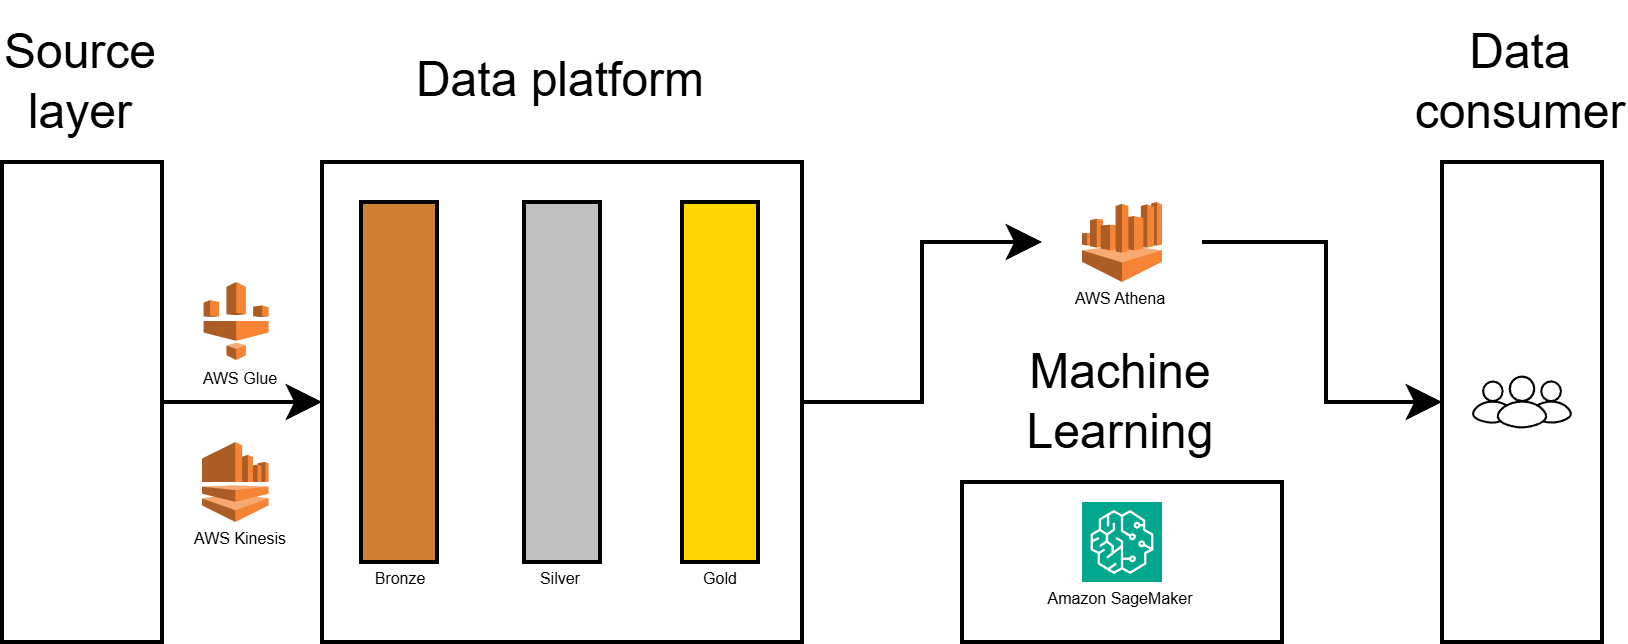
\includegraphics[width=0.5\linewidth]{images/bis11.png}
            \caption{Waterfall project phases}
        \end{figure}
    \item \textit{Agile}: the agile methodology emphasizes flexibility, iterative development, and continuous improvement. 
        Key roles in agile include:
        \begin{itemize}
            \item Product owner: responsible for defining and communicating the product goal, creating the product backlog, and prioritizing backlog items.
            \item Developers: plan the sprint, create the sprint backlog, maintain quality, and adjust plans as needed to meet the sprint goal.
            \item Scrum master: coaches the team, helps remove obstacles, and ensures focus on delivering high-value increments.
        \end{itemize}
        In agile, the work is organized into Epics (high-level product descriptions), Features (macro functionalities), Product Backlog Items (small increments delivered in one sprint), and Tasks (technical work related to a user story).
\begin{figure}[H]
    \centering
    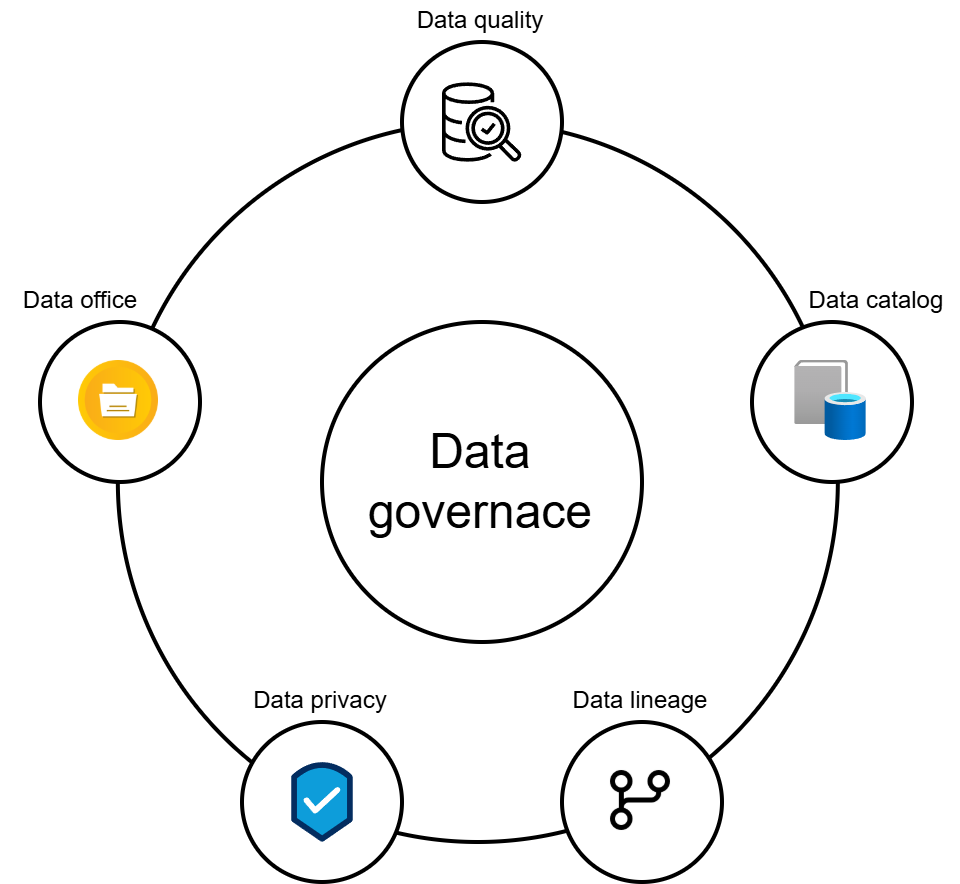
\includegraphics[width=0.5\linewidth]{images/bis12.png}
    \caption{Agile project phases}
\end{figure}
    \item \textit{Hybrid}: a hybrid methodology combines elements of both waterfall and agile, adapting to the specific needs of the project. 
        It provides flexibility while maintaining structured planning.
\end{enumerate}

\subsubsection{Requirements}
For data teams to deliver successful analytics solutions, they must first collaborate with the business to understand the business needs and the desired outcomes of the project.
A structured requirements gathering process is essential for determining the appropriate type of analysis and selecting the right solution. 
Without clear requirements, a data team cannot accurately define the scope of the project or create an effective solution.

\subsection{Data manipulation}
\begin{definition}[\textit{Data quality}]
    Data quality refers to the overall reliability, accuracy, and completeness of data. 
\end{definition}
It involves factors such as consistency, timeliness, relevance, and the absence of errors. 
High-quality data is critical for informed decision-making, effective analysis, and producing reliable outcomes across various domains like business, research, and technology. 
Ensuring data quality involves processes such as validation, cleansing, and maintaining data integrity throughout its lifecycle.

\begin{definition}[\textit{Data modeling}]
    Data modeling is the process of creating a structured representation of data to understand its relationships, constraints, and organization.
\end{definition}
\noindent Data modeling is fundamental in structuring data to ensure consistency and improve query efficiency. 
It involves defining entities (such as tables), attributes (columns), and the interconnections between them in a database. 
The goal is to guide database design and facilitate smooth, reliable data operations. 
Common types of data models include:
\begin{itemize}
    \item \textit{Data dictionaries}: a comprehensive reference that describes each data element in a system or database.
    \item \textit{Entity-relationship diagrams}: a visual representation of the structure of a relational database, illustrating the relationships between entities.
    \item \textit{Semantic models}: a logical layer that contains transformations, calculations, and relationships between data sources needed for creating reports and dashboards.
\end{itemize}
\noindent In data modeling, especially in data warehousing and business intelligence, data is typically categorized into two main types:
\begin{itemize}
    \item \textit{Dimensions}: these describe the entities in the model, such as products, people, and dates. 
        Each dimension table has a code that serves as a unique identifier and a description.
    \item \textit{Facts}: these store information related to specific observations or events, such as sales, consumption, and temperatures. 
        Fact tables typically contain the code columns of the dimensions (to create relationships with dimension tables) and numerical data.
\end{itemize}

\subsubsection{Techniques}
Normalization and denormalization are two contrasting approaches used to organize data in relational databases. 
The choice between them depends on your application's needs and goals.

\paragraph*{Normalization}
Use normalization when data integrity is the top priority. 
This approach minimizes data redundancy and helps avoid anomalies. 
It is most suitable for transactional databases where data accuracy and consistency are crucial.
Benefits of normalization:
\begin{itemize}
    \item \textit{Reduces data redundancy}: normalization splits data into separate tables to avoid duplication, saving storage space and ensuring consistency.
    \item \textit{Simplifies updates}: with normalized data, updates only need to happen in one place, minimizing the risk of inconsistent data.
    \item \textit{Supports complex relationships}: normalization allows you to represent complex relationships between entities more accurately.
    \item \textit{Normalization follows different forms}: each addressing progressively higher levels of data integrity and reduced redundancy.
\end{itemize}

\paragraph*{Denormalization}
Use denormalization when you need to optimize query performance, particularly for read-heavy workloads or reporting databases. 
It is suitable when data redundancy is acceptable if it leads to significantly faster query execution.
Benefits of denormalization:
\begin{itemize}
    \item \textit{Improves query performance}: by reducing the number of joins and minimizing the need to fetch data from multiple tables, denormalization speeds up data retrieval.
    \item \textit{Aggregations and reporting}: denormalized structures are often better suited for reporting and analytics because they simplify queries.
    \item \textit{Caching}: denormalization can make data caching easier, which can further boost performance.
\end{itemize}

In practice, many databases use a hybrid approach, selectively denormalizing certain parts of the database to improve performance while keeping other parts normalized to maintain data integrity.

\subsection{Data visualization}
Data visualization provides an intuitive way to explore and analyze data, transforming raw numbers into meaningful graphical insights.

Data visualization involves the interactive exploration and graphical representation of data, whether it's small datasets or big data, from any origin.
It enables managers and decision-makers to uncover hidden patterns, trends, and insights that might not be apparent through traditional data analysis alone.

By turning complex data into visual forms like charts, graphs, and dashboards, data visualization helps reveal crucial insights that can guide informed decision-making and drive strategic actions. 
It makes it easier to communicate complex ideas and relationships to a broader audience, improving understanding and engagement with the data.